% Original author of the front page: Jonathan Ward
\documentclass[11pt]{article} 

\usepackage{amsmath} 		% AMS Math Package
\usepackage{amsthm} 		% Theorem Formatting
\usepackage{amssymb} 		% Math symbols such as \mathbb
\usepackage{graphicx} 		% Allows for eps images
\usepackage{multicol} 		% Allows for multiple columns
\usepackage[dvips,letterpaper,margin=1in,bottom=1in]{geometry}
\usepackage{hyperref}
\usepackage{mathrsfs}
\usepackage{amsmath,amscd}
\usepackage[all,cmtip]{xy}
\usepackage{bbm}
\usepackage{fancyhdr}
\usepackage{parskip}
\usepackage{datetime}
\usepackage{tikz,pgfplots}
\usepackage{filecontents}
    \usepgfplotslibrary{groupplots}
\usetikzlibrary{decorations.pathreplacing}
\usetikzlibrary{patterns}


% %%%%%%%%%%%%%%%%%%%%%%%%%%%%%%%%%%%%%%%%%%%%%%%%%%%%%%%%
% Define bar chart colors
% %%%%%%%%%%%%%%%%%%%%%%%%%%%%%%%%%%%%%%%%%%%%%%%%%%%%%%%%
\definecolor{corLine1}{HTML}{8258FA}
\definecolor{corFill1}{HTML}{BCA9F5}

\definecolor{corLine2}{HTML}{FE2E2E}
\definecolor{corFill2}{HTML}{F78181}

\definecolor{corLine3}{HTML}{04B45F}
\definecolor{corFill3}{HTML}{00FF80}

\definecolor{corLine4}{HTML}{545454}
\definecolor{corFill4}{HTML}{9D9D9D}


\pgfplotsset{
	compat=newest,
    discard if/.style 2 args={
        x filter/.code={
            \edef\tempa{\thisrow{#1}}
            \edef\tempb{#2}
            \ifx\tempa\tempb
                \def\pgfmathresult{inf}
            \fi
        }
    },
    discard if not/.style 2 args={
        x filter/.code={
            \edef\tempa{\thisrow{#1}}
            \edef\tempb{#2}
            \ifx\tempa\tempb
            \else
                \def\pgfmathresult{inf}
            \fi
        }
    }
}





% %%%%%%%%%%%%%%%%%%%%%%%%%%%%%%%%%%%%%%%%%%%%%%%%%%%%%%%%
% Create title page
% %%%%%%%%%%%%%%%%%%%%%%%%%%%%%%%%%%%%%%%%%%%%%%%%%%%%%%%%
\newcommand*{\titleGM}{\begingroup 								% Create the command for including the title page in the document
\hbox{ 															% Horizontal box
	\hspace*{0.1\textwidth} 									% Whitespace to the left of the title page
	\rule{1pt}{\textheight} 									% Vertical line
	\hspace*{0.05\textwidth} 									% Whitespace between the vertical line and title page text
	\parbox[b]{0.75\textwidth}{ 								% Paragraph box which restricts text to less than the width of the page
		{\noindent\Huge\bfseries The Template \\}\\[2\baselineskip] 	% Title
		{\large \textit{The Topic}}\\[4\baselineskip] 					% Tagline or further description
		{\large \textsc{ Divino Cesar}}\\[0.5\baselineskip] 				% Author name
		{\large \textbf{ divcesar@gmail.com }}				 			% Author email address

		\vspace{0.5\textheight} 										% Whitespace between the title block and the publisher
		{\noindent Computer Systems Lab}\\[\baselineskip] 						% Publisher and logo
		{\noindent University of Campinas, Sao Paulo, \today.}\\[\baselineskip] 						% Publisher and logo
	}
}
\endgroup}



% %%%%%%%%%%%%%%%%%%%%%%%%%%%%%%%%%%%%%%%%%%%%%%%%%%%%%%%%
% Fancy header/footers
% %%%%%%%%%%%%%%%%%%%%%%%%%%%%%%%%%%%%%%%%%%%%%%%%%%%%%%%%
\pagestyle{fancy}
\lhead{Guides and tutorials}
\rhead{\thepage}
\lfoot{}
\rfoot{}
\cfoot{}
 
\renewcommand{\headrulewidth}{2pt}
\renewcommand{\footrulewidth}{1pt}




% %%%%%%%%%%%%%%%%%%%%%%%%%%%%%%%%%%%%%%%%%%%%%%%%%%%%%%%%
% Here begins the text
% %%%%%%%%%%%%%%%%%%%%%%%%%%%%%%%%%%%%%%%%%%%%%%%%%%%%%%%%
\begin{document}
\thispagestyle{empty}
\titleGM

\newpage
\section{Introduction}

\newpage
\section{Environment}

	\textit{\textbf{Operating System:} Linux voyager 3.13.0-35-generic \#62-Ubuntu SMP Fri Aug 15 01:58:42 UTC 2014 x86\_64 x86\_64 x86\_64 GNU\/Linux}

	\vspace{0.5cm}
	\textit{\textbf{Architecture:} Intel(R) Core(TM) i7-3630QM CPU @ 2.40GHz}
	\begin{figure}[!h]
		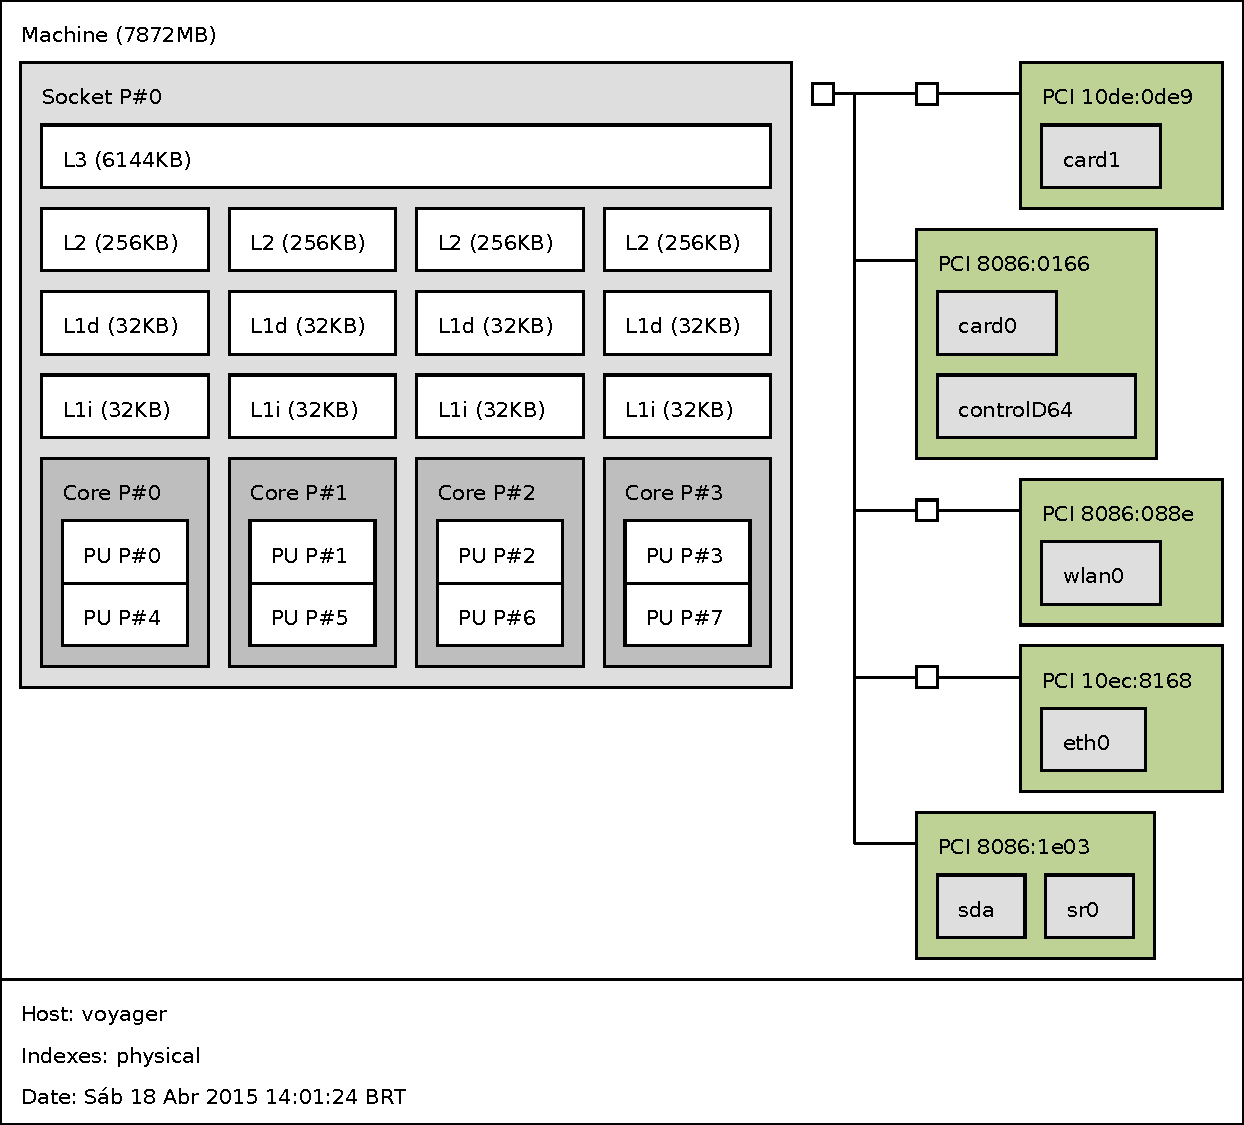
\includegraphics[width=\textwidth]{architecture}
		\caption{Diagram of the architecture were the experiments were run.}
	\end{figure}

\newpage
\section{Results}

	\subsection{First experiment}

		\textit{\textbf{Hypothesis: }Serial is faster than OMP with just one thread.}
		\vspace{0.5cm}

		In this experiment we intend to confirm that OMP with just one thread
		is slower than serial execution.

		% %%%%%%%%%%%%%%%%%%%%%%%%%%%%%%%%%%%%%%%%%%%%%%%%%%%%%%%%
		% PGF_PLOT RESULTS_TABLE
		% %%%%%%%%%%%%%%%%%%%%%%%%%%%%%%%%%%%%%%%%%%%%%%%%%%%%%%%%
		\begin{filecontents}{intel.csv}
		benchmark    	bdx 	bdx_err	  	dswp   dswp_err	  	doax   doax_err	  	doaxu doaxu_err	 
		Ferret  		1.60	0.3		 	1.60   0.3		  	1.60   0.3		  	1.60      0.3		 
		Bodytrack  		2.00	0.3		 	1.00   0.3		  	2.00   0.3		  	2.00      0.3		 
		Hmmer   		0.91	0.3		 	0.20   0.3		  	0.09   0.3		  	0.46      0.3		 
		MCF    			1.60	0.3		 	0.52   0.3		  	0.73   0.3		  	1.45      0.3		 
		Bzip2   		1.00	0.3		 	1.00   0.3		  	1.00   0.3		  	1.00      0.3		 
		H263Dec   		1.23	0.3		 	0.66   0.3		  	0.16   0.3		  	0.97      0.3		 
		KS   			0.96	0.3		 	0.92   0.3		   	0.88   0.3		  	0.94      0.3		 
		Otter   		0.67	0.3		 	0.54   0.3		   	0.52   0.3		  	0.61      0.3		 
		Geomean     	1.33	0.3		 	0.69   0.3		  	0.56   0.3		  	1.12      0.3		 
		\end{filecontents}

		\begin{figure}[!h]
			\begin{tikzpicture}
				\begin{axis}[
					ybar,
					ymajorgrids				= true,
					width  					= \textwidth,
					ylabel					= {Solubility [g per 100 g water]},
					major x tick style 	 	= transparent,
					xtick					= data,
					bar width				= 8pt,
					enlarge x limits		= 0.08,
					x tick label style		= {
						rotate	= 90,
						anchor	= east,
					},
					symbolic x coords = {
											Ferret,
											Bodytrack,
											Bzip2,
											MCF,
											Hmmer,
											H263Dec,
											KS,
											Otter,
											Geomean,
										},
					legend cell align 	 = left,
					legend image code/.code={%
						\draw[#1] (-0.1cm,-0.1cm) rectangle (0.10cm,0.2cm);
					}
				]

				\addplot [style={corLine1,fill=corFill1,mark=none}, error bars/.cd, y dir=both, y explicit]	table [x=benchmark, y=bdx, y error=bdx_err] {intel.csv};
				\addplot [style={corLine2,fill=corFill2,mark=none}, error bars/.cd, y dir=both, y explicit] table [x=benchmark, y=dswp, y error=dswp_err] {intel.csv};
				\addplot [style={corLine3,fill=corFill3,mark=none}, error bars/.cd, y dir=both, y explicit] table [x=benchmark, y=doax, y error=doax_err] {intel.csv};
				\addplot [style={corLine3,fill=corFill4,mark=none}, error bars/.cd, y dir=both, y explicit] table [x=benchmark, y=doaxu, y error=doaxu_err] {intel.csv};

				\legend{BDX, DSWP, DOAX, DOAX-U}
				\end{axis}
			\end{tikzpicture}

			\caption{First figure of the template}
		\end{figure}


	\newpage
	\subsection{Second experiment}
	
		\textit{\textbf{Hypothesis: }Serial is faster than OMP with just one thread.}
		\vspace{0.5cm}

		In this experiment we intend to confirm that OMP with just one thread
		is slower than serial execution.

		% %%%%%%%%%%%%%%%%%%%%%%%%%%%%%%%%%%%%%%%%%%%%%%%%%%%%%%%%
		% PGF_PLOT RESULTS_TABLE_1
		% %%%%%%%%%%%%%%%%%%%%%%%%%%%%%%%%%%%%%%%%%%%%%%%%%%%%%%%%
		\begin{filecontents}{arm.csv}
		x 	redi 	redi_err 	bluo 	bluo_err 
		0 	33.1 	5        	63.1 	5 
		10 	37.5 	5        	67.5 	5 
		20 	42 		5          	82 		5 
		30 	47.8 	5        	87.8 	5 
		40 	54.6 	5        	104.6 	5 
		60 	71.8 	5        	141.8 	5 
		80 	93.8 	5        	183.8 	5 
		100 124 	5       	244 	5 
		\end{filecontents}


		% %%%%%%%%%%%%%%%%%%%%%%%%%%%%%%%%%%%%%%%%%%%%%%%%%%%%%%%%
		% Figure ...
		% %%%%%%%%%%%%%%%%%%%%%%%%%%%%%%%%%%%%%%%%%%%%%%%%%%%%%%%%
		\begin{figure}[!h]
			\begin{tikzpicture}
				\begin{axis}[
					title={Temperature dependence of CuSO$_4\cdot$5H$_2$O solubility},
					xlabel={Temperature},
					ylabel={Solubility [g per 100 g water]},
					width = \textwidth,
					ymajorgrids=true,
					grid style=dashed,
				]
						 
					\addplot[color=black, mark=square] 
					plot [error bars/.cd, y dir = both, y explicit]
					table[row sep=crcr, x=x, y=redi, y error=redi_err] {arm.csv};
	
					\addplot[color=red, mark=square] 
					plot [error bars/.cd, y dir = both, y explicit]
					table[row sep=crcr, x=x, y=bluo, y error=bluo_err] {arm.csv};

					\legend{CuSO$_4\cdot$5H$_2$O, Ximphorimfola}

				\end{axis}
			\end{tikzpicture}

			\caption{First figure of the template}
		\end{figure}








\end{document}
